%! suppress、MissingLabel
%! Author = admin
%! Date = 2023/12/17

% Preamble
\documentclass[a4paper]{article}

% Packages
%基本格式
\usepackage[margin=1in]{geometry}
\usepackage[fontset=founder]{ctex}
\usepackage{anyfontsize}
\usepackage{float}
%图片
\usepackage{graphicx,caption,subcaption}
%数学公式
\usepackage{amsmath,amssymb,mathabx}
%表格
\usepackage{multirow}
%算法
\usepackage{algorithm,algorithmicx,algpseudocode}
%引用
\usepackage{hyperref}
%插入代码
\usepackage{listings}
\usepackage[usenames,dvipsnames]{xcolor}
\usepackage{mathtools}
%流程图
\usepackage{tikz}
\usetikzlibrary{positioning, shapes.geometric}

%图片路径
\graphicspath{{../figures/}}
%插入代码配置
\definecolor{mygreen}{rgb}{0,0.6,0}
\definecolor{mygray}{rgb}{0.5,0.5,0.5}
\definecolor{mymauve}{rgb}{0.58,0,0.82}
\lstset{
	\lstset{
		language=C++, % 设置语言
		basicstyle=\ttfamily, % 设置字体族
		breaklines=true, % 自动换行
		keywordstyle=\bfseries\color{NavyBlue}, % 设置关键字为粗体,颜色为 NavyBlue
		morekeywords={}, % 设置更多的关键字,用逗号分隔
		emph={self}, % 指定强调词,如果有多个,用逗号隔开
		emphstyle=\bfseries\color{Rhodamine}, % 强调词样式设置
		commentstyle=\itshape\color{black!50!white}, % 设置注释样式,斜体,浅灰色
		stringstyle=\bfseries\color{PineGreen!90!black}, % 设置字符串样式
		columns=flexible,
		numbers=left, % 显示行号在左边
		numbersep=2em, % 设置行号的具体位置
		numberstyle=\footnotesize, % 缩小行号
		frame=single, % 边框
		framesep=1em % 设置代码与边框的距离
	}

%	breakatwhitespace = false,
%	captionpos = b,
%	extendedchars = false,
%	keepspaces=true,
%	rulecolor=\color{black},
%	showspaces=false,
%	showstringspaces=false,
%	showtabs=false,
%	stepnumber=1,
%	tabsize=2,
%	title=\lstname
}

%算法配置
\renewcommand{\algorithmicrequire}{\textbf{Input:}}
\renewcommand{\algorithmicensure}{\textbf{Output:}}

\title{\textbf{数据结构实验报告}}
\author{姚苏航\qquad PB22061220}
\date{}


% Document
\begin{document}
	\maketitle


	\section{问题描述}\label{sec:des}

	\subsection{实验题目}\label{subsec:q}
	{{利用哈希表统计两源程序的相似性。}}

	\subsection{基本要求}\label{subsec:req}
	{{对于两个C语言的源程序清单,
	用哈希表的方法分别统计两程序中使用C语言关键字的情况,
	并最终按定量的计算结果,得出两份源程序的相似性。}}

	\subsection{测试数据}\label{subsec:test}
	{{事先给出的file文件夹,包含关键词表和三份源程序文件,程序之间有相近的和差别大的。
	文件内容详见附录~\ref{sec:appendix2}。}}


	\section{需求分析}\label{sec:need}

	\noindent{1.扫描给定的源程序,累计在每个源程序中 C 语言关键字出现的频度
		(为保证查找效率,建议自建哈希表的平均查找长度不大于2),
		通过这种方式扫描两个源程序,提取其特征向量。}

	\noindent{2.通过计算向量Xi和Xj的相似值来判断对应两个程序的相似性,
	相似值的判别函数计算公式为:}
	\begin{equation}
		S(X_i,X_j)=\frac{X_i^T\cdot X_j}{|X_i|\cdot|X_j|}\label{eq:equation}
	\end{equation}
	\noindent{\;\;\,\ 通过这种方式,可以初步判断两个源程序的相似性,
	如图1所示。其中 S 反映了两向量的夹角的余弦,当 S 趋近于 1 时,
	两向量夹角趋于 0 ,即两向量趋于相似,反之亦然。}
	\begin{figure}[htbp]
		\centering
		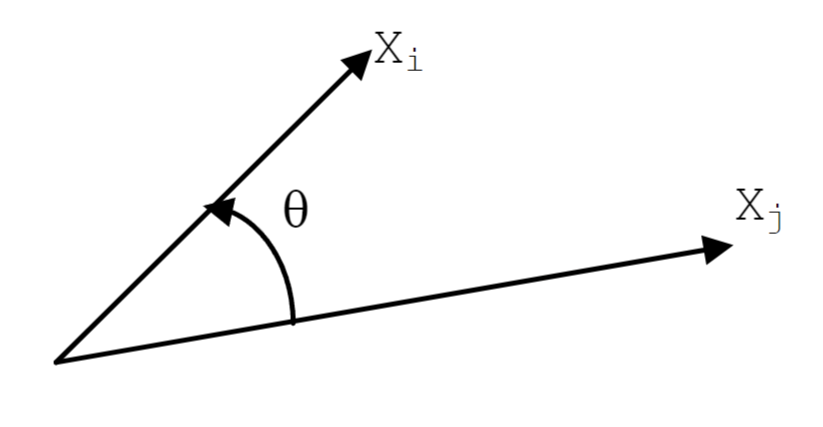
\includegraphics[height=120pt]{S}
		\caption{Similarity}
	\end{figure}

	\noindent{3.在有些情况下,S 不能很好地反映两向量的相似性,还需要进一步的考虑。
	例如,在 S 接近于 1 时,两向量的模的差距不能很好地被反映,如图2所示。
	因此引入几何距离 D ,用于反应两向量终点间的距离。}
	\begin{figure}[htbp]
		\centering
		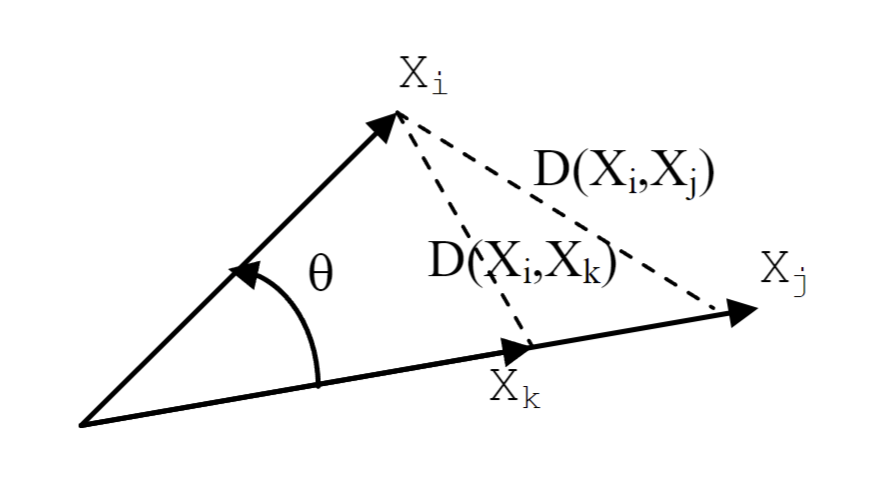
\includegraphics[height=120pt]{D}
		\caption{Distance}
	\end{figure}

	\noindent{4.通过分别比较很相近和差别很大的三个源代码,实践这种方法的有效性。}


	\section{概要设计}\label{sec:design1}

	\subsection{所用到得数据结构及其ADT}\label{subsec:adt}

	\subsection{主程序流程及其模块调用关系}\label{subsec:relate}
	\begin{tikzpicture}
		\node[draw, rounded corners](system){system};
		\node[draw, rounded corners,below=5pt of system](start){start};
		\node[draw, below=of start](CH){CreateHash//创建哈希表};
		\node[draw, below=of CH](V){CreateEigenvector};
		\node[draw, below=of V](S){SAsses//计算相似度};
		\node[draw, below=of S](D){DAsses//计算几何距离};
		\node[draw, rounded corners, below=20pt of D](end){End};

		\draw[->] (start)  -- (CH);
		\draw[->] (CH) -- (V);
		\draw[->] (V) -- (S);
		\draw[->] (S) -- (D);
		\draw[->] (D) -- (end);


		\node[draw, rounded corners,right=120pt of system](CV){CreateEigenvector};
		\node[draw, rounded corners,below=5pt of CV](start1){start};
		\node[draw, ellipse,below=of start1](L){While};
		\node[left =50pt of L](temp){};
		\node[draw, diamond, aspect=2, below=of L](eof){!fin.eof()};
		\node[draw, below=of eof](RW){ReadWord//读取单词};
		\node[draw, below=of RW](SH){SearchHash//查找表};
		\node[left =23pt of SH](temp1){};
		\node[draw, right=45pt of eof](EV){Eigenvector//得到特征向量};
		\node[draw, rounded corners, below=20pt of EV](end1){End};

		\draw[->] (start1)  -- (L);
		\draw[->] (L)  -- (eof);
		\draw[->] (eof) -- node[left]  {Yes} (RW);
		\draw[->] (RW)  -- (SH);
		\draw[->] (SH)  --(temp|-SH)--(temp)--(L);
		\draw[->] (SH)  --(temp1)--(temp1|-L)--(L);
		\draw[->] (eof) -- node[above] {No}  (EV);
		\draw[->] (EV) -- (end1);

	\end{tikzpicture}


	\section{详细设计}\label{sec:design2}

	\subsection{实现概要设计中的数据结构ADT}\label{subsec:adt2}
	\begin{lstlisting}[caption={},label={lst:lstlisting}][H]
        typedef struct {
          KeyType key;
          Datatype Data;  // 记录关键字出现的次数
        } ElemType;       // 包含关键字和数据

        typedef struct LHNode {  // 哈希表结点
          ElemType data;         // 查找表单元
          LHNode *next;          // 后继
        } *LHptr;

        typedef struct {
          LHptr *elem;
          int count;   // 记录数
        int size;    // 容量
        } LHashTable;  // 链地址存储法
	\end{lstlisting}

	\subsection{实现每个操作的伪码,重点语句加注释}\label{subsec:explain}

	\subsubsection{哈希表的创建与查找}
	\begin{algorithm}[H]
		\caption{创建哈希表}
		\begin{algorithmic}[1] %每行显示行号
			\Function {CreateHash}{$LHashTable\ \&H$}
				\State $ifstream fin(“../file/keywords.txt”, ios \dblcolon in)$;
				\State $keyword[0] \gets new\ char[30]$;
				\For{$each\ i\ in\ [1,22]$}
					\State $keyword[i] \gets new\ char[10]$;\Comment{为每个节点分配空间}
				\EndFor

				\State $fin.get(keyword[0], 26)$;\Comment{将无用内容读入keyword[0],关键字从1开始存储}
				\State $i\gets 1$,$j\gets 0$;
				\While{$!fin.eof()$}
					\State $fin.get(ch)$;
					\If{$ch >= 97 \&\& ch <= 122$}
						\Comment{判断是否为需要读取的关键词}
						\State $keyword[i][j] \gets  ch$;\Comment{读取关键词}
						\State $j++$;
					\Else
						\State $keyword[i][j] \gets '\backslash 0'$;
						\State $j \gets  0$,$i++$;\Comment{为读取下一个关键词做准备}
					\EndIf
				\EndWhile

				\State $H.size \gets  43;H.count \gets  0$
				\State $H.elem \gets  new\ LHptr[H.size]$\Comment{初始化为所有结点指针的头指针}
				\For{$each\ i\ in\ [0,H.size-1]$}
					\State $H.elem[i] \gets  new\ LHNode;$ \Comment{为单个结点分配空间}
					\State $H.elem[i]->next \gets  nullptr;$
				\EndFor
				\For {$each\ i\ in\ [1,17]$}
					\State $n \gets  Hash(keyword[i])$;
					\State $p \gets  new\ LHNode;p->data.key \gets  new\ char[10];$\Comment{分配空间}
					\State $p->next \gets  nullptr;p->data.Data \gets  0;$\Comment{计数}
					\State $p->data.key \gets keyword[i]$\Comment{记录key值}
					\If{!$H.elem[n]->next$}
						\State $H.elem[n]->next \gets  p$;
					\Else
						\State $p->next \gets  H.elem[n]->next$;
						\State $H.elem[n]->next \gets  p$;
					\EndIf
				\EndFor
				\State $fin.close();$
			\EndFunction
		\end{algorithmic}\label{alg:algorithm}
	\end{algorithm}

	\begin{algorithm}[H]
		\caption{查找哈希表}
		\begin{algorithmic}[1] %每行显示行号
			\Function {SearchHash}{$LHashTable\ H, int\ n, KeyType\ key$}
				\State $p \gets H.elem[n]->next$;
				\While{$p$}
					\If{!strcmp(key, p->data.key)}
						\Comment{等于则返回0}
						\State $p->data.Data++$;
						\State break;
					\EndIf
					\State $p \gets p->next$;
				\EndWhile
			\EndFunction
		\end{algorithmic}\label{alg:algorithm2}
	\end{algorithm}

	\subsubsection{向量的生成与运算}
	\begin{algorithm}[H]
		\caption{读取文件生成向量}
		\begin{algorithmic}[1] %每行显示行号
			\Function {CreateEigenvector}{$LHashTable\ H, int\ X[], const\ string\&\ FileAddress$}
				\State $InitHash()$;\Comment{初始化哈希表}
				\While{$!fin.eof()$}
					\State $ReadWord()$;\Comment{读取单词};
					\State $n \gets Hash()$;\Comment{计算哈希值};
					\State $SearchHash()$;\Comment{搜索哈希表};
				\EndWhile
				\For{$each\ i\ in\ [0,43)]$}
					\State $p \gets H.elem[i]->next$;
					\While{$p$}
						\State $X[j++] \gets p->data.Data$;\Comment{用哈希表的记录生成特征向量}
						\State $p \gets p->next$;
					\EndWhile
				\EndFor
				\State $fin.close()$;
			\EndFunction
		\end{algorithmic}\label{alg:algorithm3}
	\end{algorithm}

	\begin{algorithm}[H]
		\caption{计算几何距离}
		\begin{algorithmic}[1] %每行显示行号
			\Function {DAsses}{$const\ int\ X1[],\ const\ int\ X2[]$}
				\State $k,i,m \gets 0$;
				\For{$each\ i\ in\ [0,16)$}
					\State $m += (X1[i] - X2[i]) * (X1[i] - X2[i]);$;\Comment{计算X1和X2的差}
				\EndFor
				\State $k = sqrt(m)$;\Comment{计算几何距离D}
				\Return $k$;
			\EndFunction
		\end{algorithmic}\label{alg:algorithm4}
	\end{algorithm}

	\begin{algorithm}[H]
		\caption{计算相似度}
		\begin{algorithmic}[1] %每行显示行号
			\Function {SAsses}{$const\ int\ X1[],\ const\ int\ X2[]$}
				\State $n1,n2,i,m \gets 0$;
				\For{$each\ i\ in\ [0,16)$}
					\State $m += X1[i] * X2[i]$;\Comment{计算X1和X2的点积}
					\State $n1 += X1[i] * X1[i]$;
					\State $n2 += X2[i] * X2[i]$;
				\EndFor
				\State $n1 = sqrt(n1)$;\Comment{计算X1的模}
				\State $n2 = sqrt(n2)$;\Comment{计算X2的模}\\
				\Return $m /= n1 * n2$;\Comment{返回相似度S}
			\EndFunction
		\end{algorithmic}\label{alg:algorithm5}
	\end{algorithm}

	\subsection{主程序和其他模块的伪码}\label{subsec:code2}
	\begin{algorithm}[H]
		\caption{判断相似性}
		\begin{algorithmic}[1] %每行显示行号
			\Function {system}{$void$}
				\State $CreateHash(H)$;\Comment{根据给定关键词创建哈希表}
				\State $CreateEigenvector(H, SimVec, "../file/similar.c")$;\Comment{读取程序生成特征向量}
				\State $CreateEigenvector(H, DifVec, "../file/different.c")$;
				\State $CreateEigenvector(H, MainVec, "../file/main.c")$;
				\State $Similarity \gets SAsses(SimVec, MainVec)$;\Comment{计算相似度S和几何距离D}
				\State $Distance \gets DAsses(SimVec, MainVec)$;
				\State $Similarity \gets SAsses(DifVec, MainVec)$;
				\State $Distance \gets DAsses(DifVec, MainVec)$;
			\EndFunction
		\end{algorithmic}\label{alg:algorithm6}
	\end{algorithm}


	\section{调试分析}\label{sec:debug}

	\subsection{问题分析与体会}\label{subsec:analysis}
	{{本项目工程主要分为两个部分。
	第一部分是哈希表的创建和查找,第二部分是根据查找结果得到向量以及对向量的数学计算等处理。}}

	{在这两部分中,文件的读取和写入是必不可少的,因此,对文件的读写操作是调试的重点。
	在本实验中,根据给定的文件,选用适当的函数读取文件,并且注意想要获取的内容间分隔符的处理,
	是第一个难点,也是调试的重点。此外,文件读取状态的判断也是一个重点。}

	{{在正确地读取文件内容后,如何处理向量也是实验重点。
	在一开始,只是简单地将每个读取的向量的处理步骤转换成代码,造成了代码臃肿,复用性差,并且难以调试的问题。
	通过对代码的重构和优化,将向量的处理步骤封装成通用的函数,使得代码的复用性大大提高,
	并且易于调试,在实验过程中数学运算的错误也更易发现。}}

	{{在本次实验中,注释发挥了重要的作用。通过对一些细节操作的注释,大幅加快了调试的速度。在遇到问题时能够很快找到解决方案。
	注释也大幅提高了代码可读性,在优化代码时,注释作为参考,指明了数据初始化的状态,重要操作的目的,方便了后期的维护与修改。}}

	{{通过这次实验,我锻炼了自己处理多个文件的能力,
	认识了注释等好的编程习惯的重要性,提升了自己对非单一文件的项目工程的函数编写封装思路的理解。
	它不仅加深了我对哈希表的认识,了解了哈希表在查重方面的应用,还提高了自己代码的编写能力,能够更好更快地写出容易理解且便于调试的代码。}}

	\subsection{时空复杂度分析}\label{subsec:analysis2}


	\section{使用说明}\label{sec:instrut}
	{{用户将事先准备好的关键词表(keyword.txt)和需要统计相似性的程序放入file文件夹中,
	运行时程序将通过关键词表建立哈希表,并通过查找哈希表构建两程序的向量,
	最后通过判别函数计算两程序相似性和向量的几何距离。}}

	{{在本项目中,使用事先给出的测试数据,
	准备三个编译和运行都无误的C程序,程序之间有相近的和差别大的,
	通过similar.c和different.c两个程序与main.c进行比较,
	可以直观展现出比较的效果。}}


	\section{测试结果}\label{sec:result}

	\subsection{输入数据}\label{subsec:in}
	{{输入数据从给出的测试文件中读取,
	读取keyword.txt文件生成哈希表,
	再分别读取main.c,similar.c,different.c并进行比较。}}

	\subsection{输出数据}\label{subsec:out}
	\noindent{输出结果显示在终端,内容如下:}

	\noindent{X\_(../file/similar.c):}

	\noindent{0 1 1 4 0 1 0 3 3 1 2 1 2 0 1 1 4}

	\noindent{X\_(../file/different.c):}

	\noindent{0 1 0 1 0 0 1 2 1 0 3 0 0 0 1 3 2}

	\noindent{X\_(../file/main.c):}

	\noindent{0 1 1 3 0 1 0 3 2 1 2 1 2 0 1 1 4}

	\noindent{ }

	\noindent{S\_(Sim\&Main):0.988174}

	\noindent{D\_(Sim\&Main):1.41421}

	\noindent{ }

	\noindent{S\_(Dif\&Main):0.740121}

	\noindent{D\_(Dif\&Main):4.89898}


	\appendix


	\section{实验源代码文件}\label{sec:appendix1}
	{{为方便查看,附录中的链接文件均为txt格式}}

	\href{../exp6/define.h.txt}{\underline{define.h}}

	\href{../exp6/main.cpp.txt}{\underline{main.cpp}}

	\href{../exp6/OpenHashing.h.txt}{\underline{OpenHashing.h}}

	\href{../exp6/OpenHashing.cpp.txt}{\underline{OpenHashing.cpp}}

	\href{../exp6/system.h.txt}{\underline{system.h}}

	\href{../exp6/system.cpp.txt}{\underline{system.cpp}}

	\href{../exp6/SimAsses.h.txt}{\underline{SimAsses.h}}

	\href{../exp6/SimAsses.cpp.txt}{\underline{SimAsses.cpp}}


	\section{实验用测试文件}\label{sec:appendix2}
	\href{../exp6/file/main.c.txt}{\underline{main.c}}

	\href{../exp6/file/different.c.txt}{\underline{different.c}}

	\href{../exp6/file/similar.c.txt}{\underline{similar.c}}

	\href{../exp6/file/keyword.txt}{\underline{keyword.txt}}


\end{document}


%    \begin{algorithm}
%        \caption{开散列哈希表}
%        \begin{algorithmic}[1] %每行显示行号
%            \Require $Array$数组,$n$数组大小
%            \Ensure 逆序数
%            \Function {MergerSort}{$Array, left, right$}
%                \State $result \gets 0$
%                \If {$left < right$}
%                    \State $middle \gets (left + right) / 2$
%                    \State $result \gets result +$ \Call{MergerSort}{$Array, left, middle$}
%                    \State $result \gets result +$ \Call{MergerSort}{$Array, middle, right$}
%                    \State $result \gets result +$ \Call{Merger}{$Array,left,middle,right$}
%                \EndIf
%                \State \Return{$result$}
%            \EndFunction
%            \State
%            \Function{Merger}{$Array, left, middle, right$}
%                \State $i\gets left$
%                \State $j\gets middle$
%                \State $k\gets 0$
%                \State $result \gets 0$
%                \While{$i<middle$ \textbf{and} $j<right$}
%                    \If{$Array[i]<Array[j]$}
%                        \State $B[k++]\gets Array[i++]$
%                    \Else
%                        \State $B[k++] \gets Array[j++]$
%                        \State $result \gets result + (middle - i)$
%                    \EndIf
%                \EndWhile
%                \While{$i<middle$}
%                    \State $B[k++] \gets Array[i++]$
%                \EndWhile
%                \While{$j<right$}
%                    \State $B[k++] \gets Array[j++]$
%                \EndWhile
%                \For{$i = 0 \to k-1$}
%                    \State $Array[left + i] \gets B[i]$
%                \EndFor
%                \State \Return{$result$}
%            \EndFunction
%        \end{algorithmic}\label{alg:algorithm2}
%    \end{algorithm}
